% file          : doc_tex/basic/Triangulation_3/Triang3.tex
% revision      : $Id$
%
% author(s)     : Monique Teillaud <Monique.Teillaud@sophia.inria.fr>

\begin{ccTexOnly}
%\vspace*{-1cm}
\begin{center}
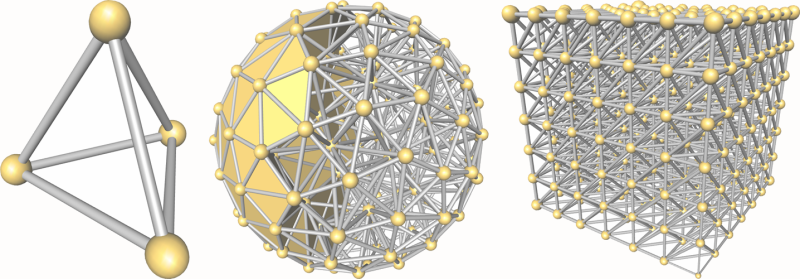
\includegraphics[width=15cm]{Triangulation_3/triangulation3}
\end{center}
\end{ccTexOnly}
\begin{ccHtmlOnly}
<img border=0 src="./triangulation3.png" alt="3D triangulation picture">
\end{ccHtmlOnly}

The basic 3D-triangulation class of \cgal\ is primarily designed to
represent the triangulations of a set of points $A$ in $\R^3$.  It is
a partition of the convex hull of {$A$} into tetrahedra whose vertices
are the points of {$A$}.  Together with the unbounded cell having the
convex hull boundary as its frontier, the triangulation forms a
partition of $\R^3$. Its cells ($3$-faces) are such that two cells
either do not intersect or share a common facet ($2$-face), edge
($1$-face) or vertex ($0$-face).

\section{Representation\label{Triangulation3-sec-intro}}

In order to deal
only with tetrahedra, which is convenient for many applications, the
unbounded cell can be subdivided into tetrahedra by considering that
each convex hull facet is incident to an \ccc{infinite cell} having as
fourth vertex an auxiliary vertex called the \ccc{infinite vertex}.  In
that way, each facet is incident to exactly two cells and special cases
at the boundary of the convex hull are simple to deal with.

The class \ccc{Triangulation_3<TriangulationTraits_3,TriangulationDataStructure_3>} of \cgal\ implements this
point of view and therefore considers the triangulation of the set
of points as a set of finite and infinite tetrahedra.  Notice that the
infinite vertex has no significant coordinates and that no
geometric predicate can be applied on it.

A triangulation is a collection of vertices and cells that are linked
together through incidence and adjacency relations. Each cell gives
access to its four incident vertices and to its four adjacent
cells. Each vertex gives access to one of its incident cells.

The four vertices of a cell are indexed with 0, 1, 2 and 3 in positive
orientation, the positive orientation being defined by the orientation
of the underlying Euclidean space $\R^3$ (see
Figure~\ref{Triangulation3-fig-orient}). The neighbors of a cell are also
indexed with 0, 1, 2, 3 in such a way that the neighbor indexed by $i$
is opposite to the vertex with the same index. 

\begin{figure}[htbp]
\begin{ccTexOnly}
\begin{center} 
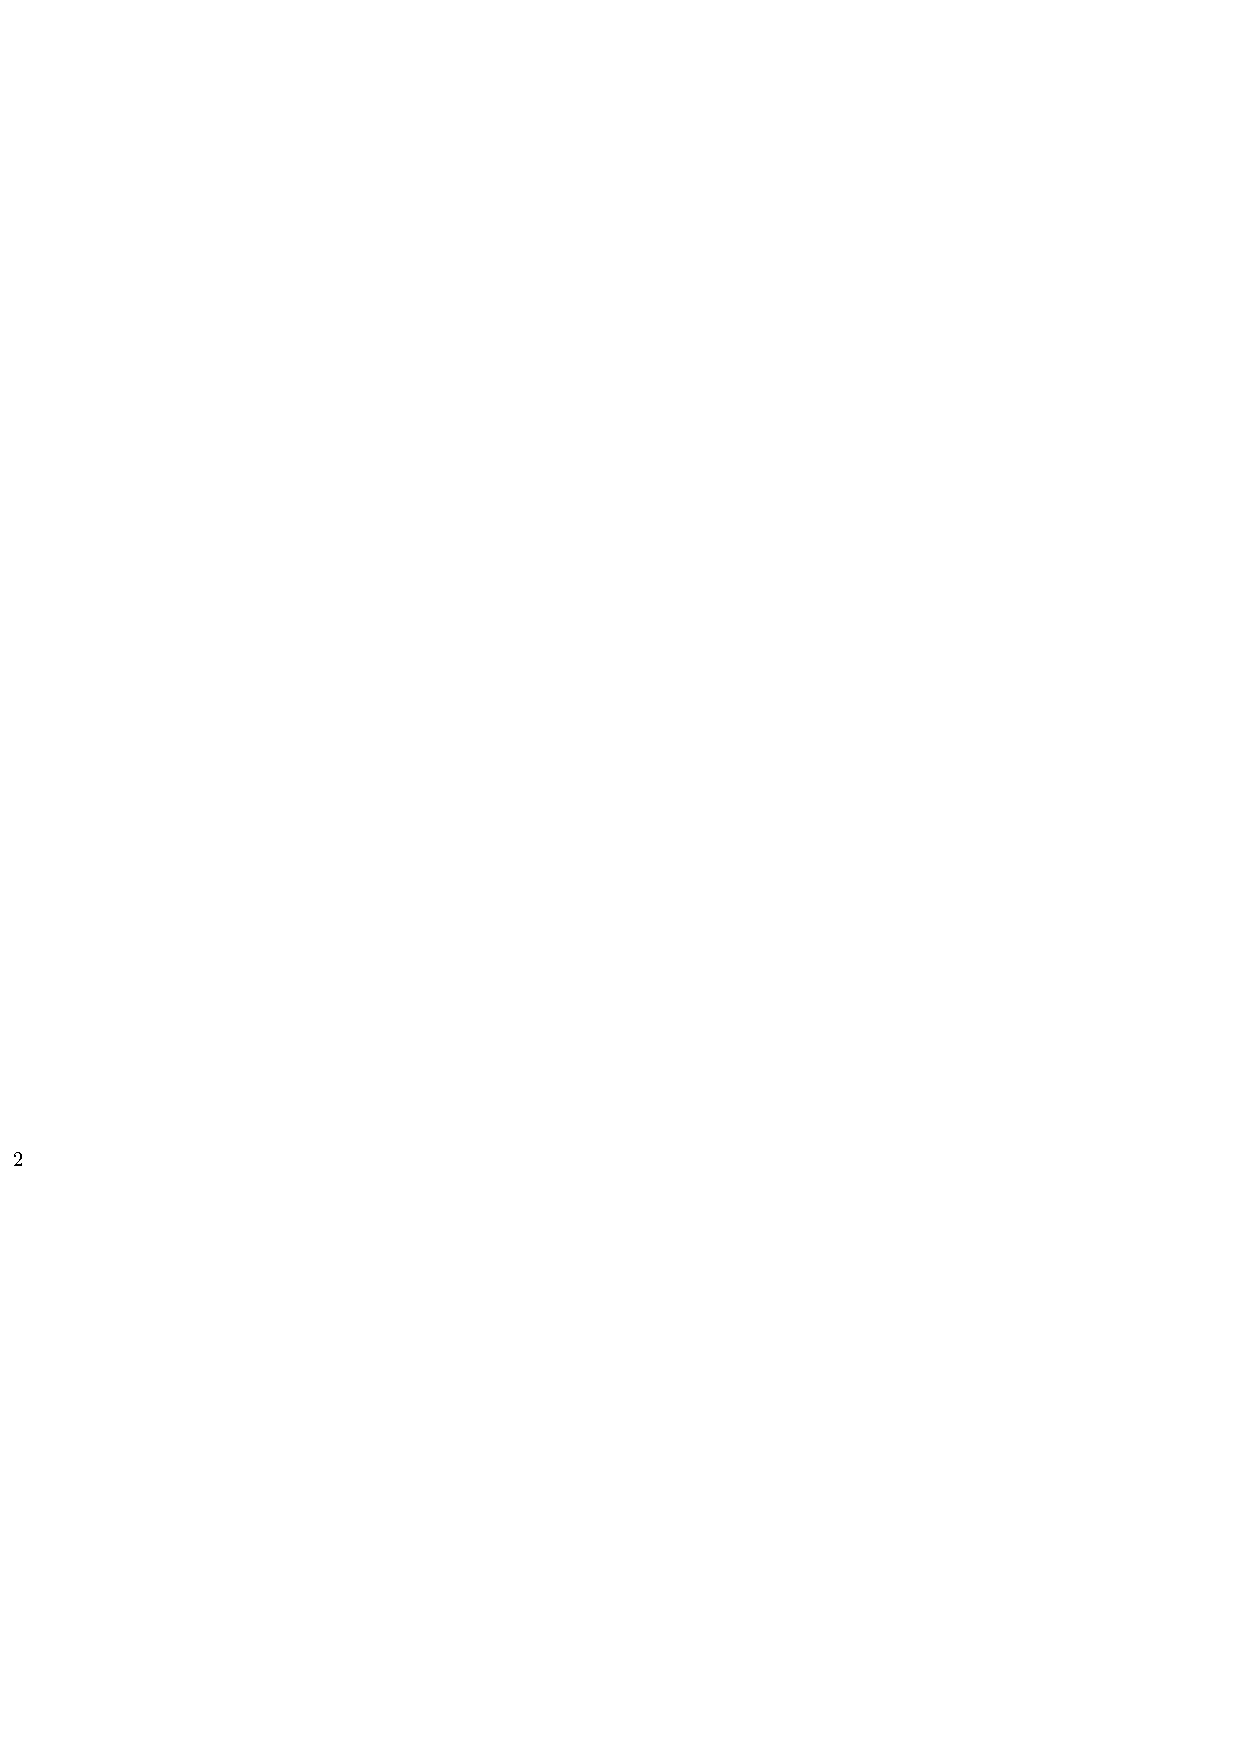
\includegraphics{Triangulation_3/orient} 
\end{center}
\end{ccTexOnly}
\begin{ccHtmlOnly}
<CENTER>
<img border=0 src="./orient.gif" align=middle alt="Orientation of a cell 
(3-dimensional case)">
</CENTER>
\end{ccHtmlOnly}
\caption{Orientation of a cell (3-dimensional case).
\label{Triangulation3-fig-orient}}
\end{figure} 

As in the underlying combinatorial triangulation (see
Chapter~\ref{chapter-TDS3}), edges ($1$-faces) and facets ($2$-faces)
are not explicitly 
represented: a facet is given by a cell and an index (the facet
\ccc{i} of a cell \ccc{c} is the facet of \ccc{c} that is opposite to
the vertex with index \ccc{i}) and an edge is given by a cell and two
indices (the edge \ccc{(i,j)} of a cell \ccc{c} is the edge whose
endpoints are the vertices of \ccc{c} with indices \ccc{i} and
\ccc{j}). See Figure~\ref{TDS3-fig-repres}.  

\paragraph{Degenerate Dimensions}
The class \ccc{Triangulation_3} can also deal with
triangulations whose dimension $d$ is less than~3. A triangulation of a
set of points in $\R^d$ covers the whole space $\R^d$ and consists of
cells having $d+1$ vertices: some of them are infinite, they are
obtained by linking the additional infinite vertex to each facet of
the convex hull of the points.
\begin{itemize}
\item {} \emph{dimension 2:} when a triangulation only contains
coplanar points (which is the case when there are only three points), 
it consists of triangular faces.
\item {} \emph{dimension 1:} the triangulation contains only collinear 
points (which is the case when there are only two points), it consists
of edges.
\item {} \emph{dimension 0:} the triangulation contains only one
finite point.
\item {} \emph{dimension -1:} this is a convention to handle the case
when the only vertex of the triangulation is the infinite one.
\end{itemize} 

The same cell class is used in all cases: triangular faces in
2D can be considered as degenerate cells, having only three vertices
(resp. neighbors) numbered $(0,1,2)$;
edges in 1D have only two vertices (resp. neighbors) numbered $0$ and $1$. 

The implicit representation of facets (resp. edges) still holds
for degenerate dimensions (\textit{i.e.} dimensions $<3$): in
dimension~2, each cell has only one facet of index 3, and 3 edges
$(0,1)$, $(1,2)$ and $(2,0)$; in dimension~1, each cell has one edge
$(0,1)$.  

\paragraph{Validity}
A triangulation of $\R^3$ is said to be \ccc{locally valid} iff

{\bf (a)-(b)} Its underlying combinatorial graph, the triangulation
data structure, is \ccc{locally valid} 
(see Section~\ref{TDS3-sec-intro} of Chapter~\ref{chapter-TDS3})\\
{\bf (c)} Any cell has its vertices ordered according to positive
orientation. See Figure~\ref{Triangulation3-fig-orient}.

When the triangulation is degenerated into a triangulation of
dimension~2, the  geometric validity reduces to:

{\bf (c-2D)} For any two adjacent triangles $(u,v,w_1)$ and $(u,v,w_2)$ with
common edge $(u,v)$, $w_1$ and $w_2$ lie on opposite sides of $(u,v)$
in the plane.

When all the points are collinear, this condition becomes:

{\bf (c-1D)} For any two adjacent edges $(u,v)$ and $(v,w)$, $u$ and
$w$ lie on opposite sides of the common vertex $v$ on the line.

The \ccc{is_valid()} method provided in \ccc{Triangulation_3} checks
the local validity of a given triangulation. This does not always
ensure global validity \cite{mnssssu-cgpvg-96,dlpt-ccpps-98} but it is 
sufficient for practical cases.


\section{Delaunay Triangulation} 

The class \ccc{Delaunay_triangulation_3} represents a three-dimensional
Delaunay triangulation.

Delaunay triangulations have the specific \textit{empty sphere property},
that is, the circumscribing sphere of each cell of such a triangulation
does not contain any other vertex of the triangulation in its interior.
These triangulations are uniquely defined except in degenerate cases
where five points are co-spherical.  Note however that the \cgal\ implementation
computes a unique triangulation even in these cases.

This implementation is fully dynamic: it supports insertions of points, vertex removals
and displacements of points.


\section{Regular Triangulation\label{Triangulation3-sec-class-Regulartriangulation}}

The class \ccc{Regular_triangulation_3} implements incremental regular
triangulations, also known as weighted Delaunay triangulations.

Let ${S}^{(w)}$ be a set of weighted points in $\R^3$. Let
${p}^{(w)}=(p,w_p), p\in\R^3, w_p\in\R$ and 
${z}^{(w)}=(z,w_z), z\in\R^3, w_z\in\R$ be two weighted points. 
A weighted point
${p}^{(w)}=(p,w_p)$ can also be seen as a sphere of center $p$ and
radius $\sqrt{w_p}$. 
The \textit{power product} between ${p}^{(w)}$ and ${z}^{(w)}$ is
defined as 
\[\Pi({p}^{(w)},{z}^{(w)}) = {\|{p-z}\|^2-w_p-w_z}\]
where $\|{p-z}\|$ is the Euclidean distance between $p$ and $z$. 
 ${p}^{(w)}$ and ${z}^{(w)}$
are said to be \textit{orthogonal} iff $\Pi{({p}^{(w)},{z}^{(w)})}
= 0$ (see Figure~\ref{Triangulation3-fig-ortho}).

\begin{figure}[htbp]
\begin{ccTexOnly}
\begin{center} 
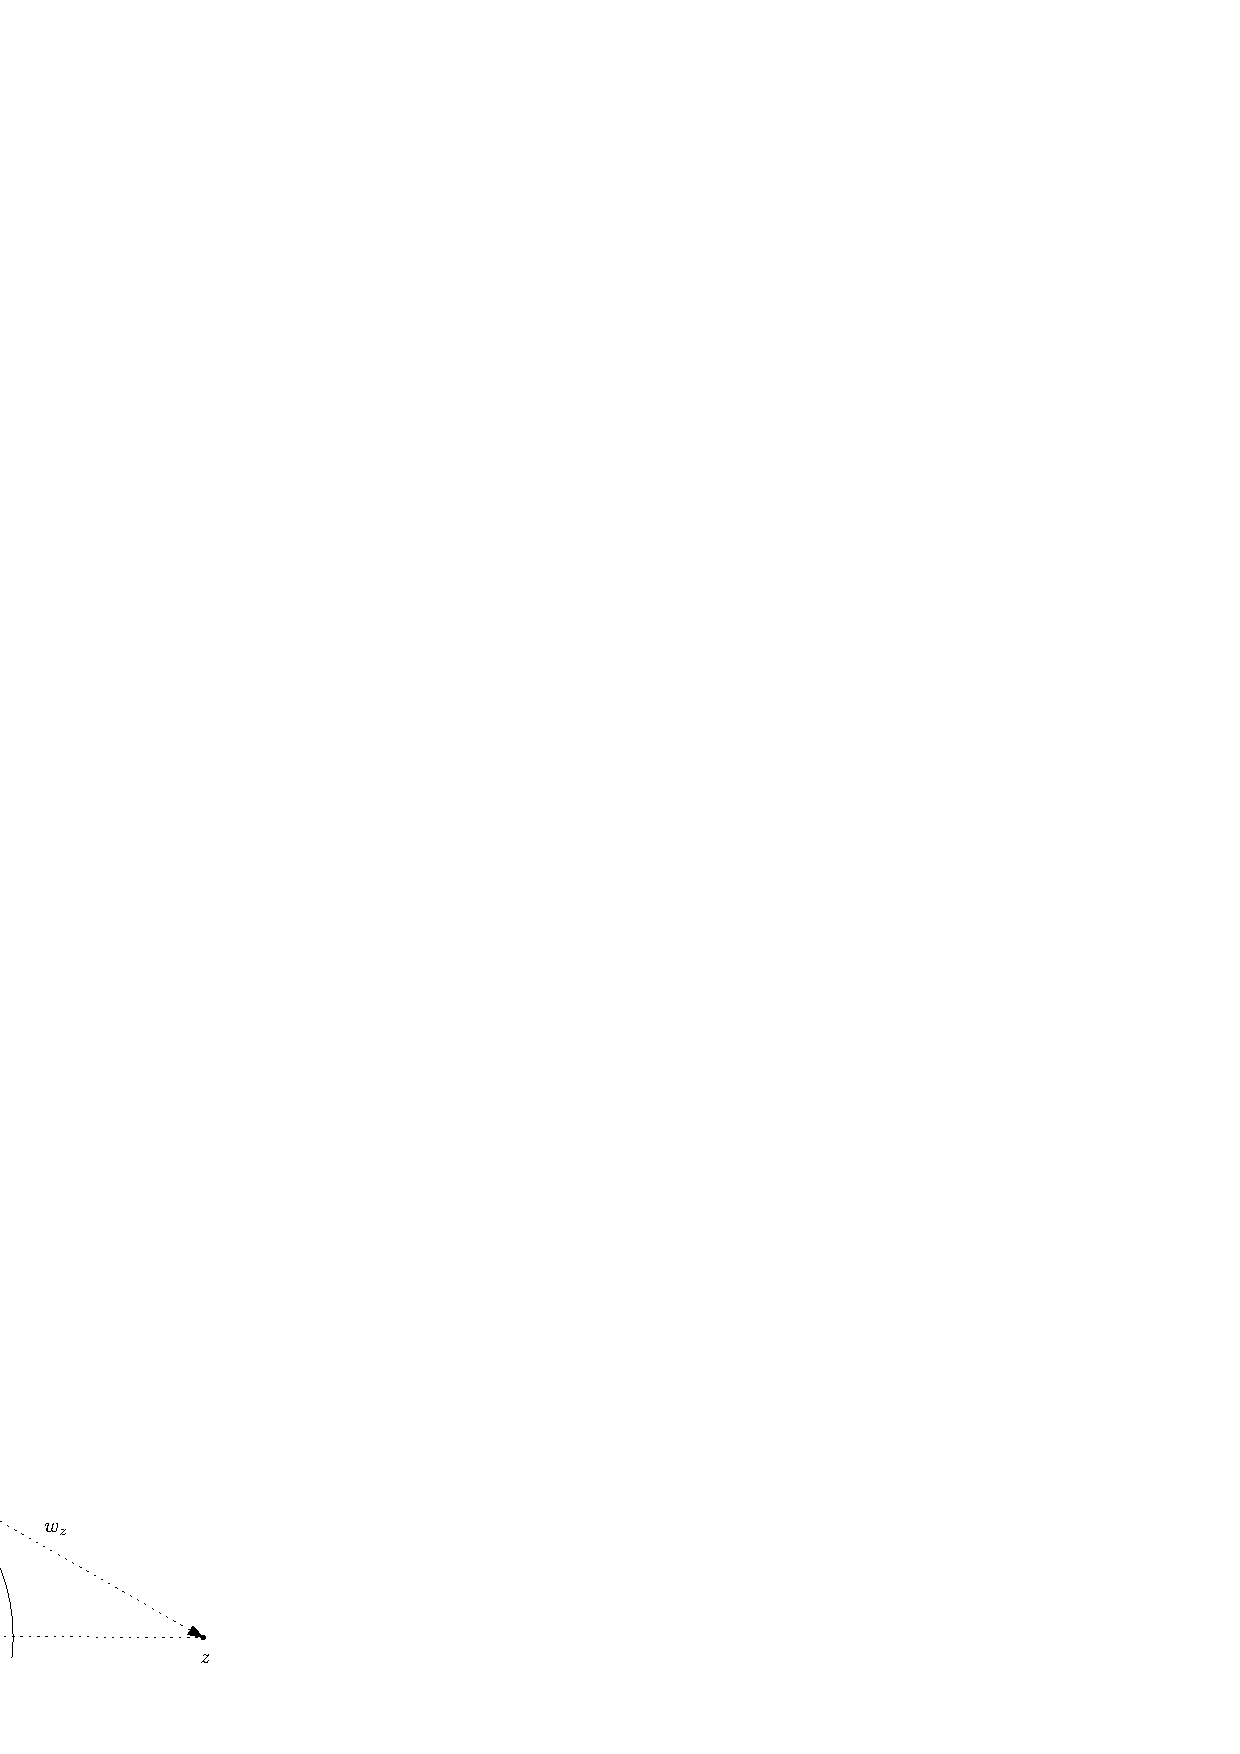
\includegraphics{Triangulation_3/ortho} 
\end{center}
\end{ccTexOnly}
\begin{ccHtmlOnly}
<CENTER>
<img border=0 src="./ortho.gif" align=middle alt="Orthogonal weighted
points (picture in 2D)"> 
</CENTER>
\end{ccHtmlOnly}
\caption{Orthogonal weighted points (picture in 2D).
\label{Triangulation3-fig-ortho}}
\end{figure} 

Four weighted points have a unique common orthogonal weighted point
called the \textit{power sphere}.  The weighted point orthogonal to
three weighted points in the plane defined by these three points is
called the \textit{power circle}. The
\textit{power segment} will denote the weighted point orthogonal to
two weighted points on the line defined by these two points.

A sphere ${z}^{(w)}$ is said to be
\textit{regular} if $\forall {p}^{(w)}\in{S}^{(w)},
\Pi{({p}^{(w)},{z}^{(w)})}\geq 0$.

A triangulation of ${S}^{(w)}$ is \textit{regular} if the power spheres
of all simplices are regular. 

The regular triangulation of
${S}^{(w)}$ is in fact the projection onto $\R^3$ of the convex hull 
of the four-dimensional points $(p,\|p-O\|^2-w_p),$ for
${p}^{(w)}=(p,w_p)\in{S}^{(w)}$. 
Note that all points of ${S}^{(w)}$ do not
necessarily appear as vertices of the regular
triangulation. To know more about regular triangulations, see for
example \cite{es-itfwr-96}. 

When all weights are 0, power spheres are nothing more than
circumscribing spheres, and the regular triangulation is exactly the
Delaunay triangulation.

The implementation of 3D regular triangulation supports insertions of weighted points, and vertex removals. Displacements are not supported in the current implementation.

\section{Software Design\label{Triangulation3-sec-design}}

The main classes \ccc{Triangulation_3}, \ccc{Delaunay_triangulation_3} and
\ccc{Regular_triangulation_3} are connected to each other by the
derivation diagram shown in Figure~\ref{t3_derivation}.  This diagram
also shows another class: \ccc{Triangulation_utils_3}\lcTex{
(\ccRefPage{CGAL::Triangulation_utils_3})}, which provides
a set of tools operating on the indices of vertices in cells.

\begin{figure}[htbp]
\begin{ccTexOnly}
\begin{center} 
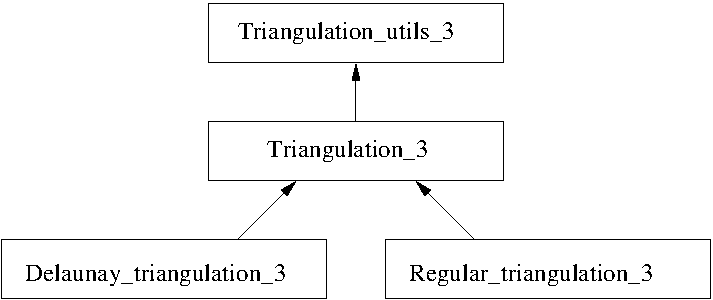
\includegraphics{Triangulation_3/derivation} 
\end{center}
\end{ccTexOnly}
\begin{ccHtmlOnly}
<CENTER>
<img border=0 src="./derivation.gif" align=middle
alt="Derivation diagram of the 3D triangulation classes"> 
</CENTER>
\end{ccHtmlOnly}
\caption{Derivation diagram of the 3D triangulation classes.
\label{t3_derivation}}
\end{figure} 

The three main classes (\ccc{Triangulation_3}, \ccc{Delaunay_triangulation_3}
and \ccc{Regular_triangulation_3}) provide high-level geometric functionality
such as location of a point in the triangulation~\cite{cgal:dpt-wt-02}, insertion
and possibly removal of a point~\cite{cgal:dt-pvr3d-03}, and are responsible for the
geometric validity.  They are built as layers on top of a triangulation data
structure, which stores their combinatorial structure.  This separation between
the geometry and the combinatorics is reflected in the software design by the
fact that these three triangulation classes take the following template parameters :

\begin{itemize}
\item {} the \textbf{geometric traits} class, which provides the type of points
to use as well as the elementary operations on them (predicates and
constructions).  The concepts for these parameters are described in more
details in Section~\ref{Triangulation3-sec-Traits}\lcTex{ and in 
\ccRefPage{TriangulationTraits_3}}.
\item {} the \textbf{triangulation data structure} class, which stores their
combinatorial structure, described in Section~\ref{TDS3-sec-design} of
Chapter~\ref{chapter-TDS3}.
\item {} the \textbf{location policy} tag, which is supported only by the Delaunay
triangulation class, described in Section~\ref{Triangulation3-sec-locpol}.
\end{itemize}


\subsection{The Geometric Traits Parameter\label{Triangulation3-sec-Traits}}

The first template parameter of the triangulation class
\ccc{Triangulation_3<TriangulationTraits_3, TriangulationDataStructure_3>}
is the geometric traits class, described by the concept
\ccc{TriangulationTraits_3}.  It must define the types of the geometric objects
(points, segments, triangles and tetrahedra) forming the triangulation together
with a few geometric predicates on these objects: orientation in space,
orientation in case of coplanar points, order of collinear points.

In addition to the requirements described before, the geometric traits
class of \ccc{Delaunay_triangulation_3} must define predicates to test for the
\textit{empty sphere property}.  It is described by the concept
\ccc{DelaunayTriangulationTraits_3}, which refines \ccc{TriangulationTraits_3}.

The kernels provided by \cgal: \ccc{Cartesian}, \ccc{Homogeneous},
\ccc{Simple_cartesian}, \ccc{Simple_homogeneous} and
\ccc{Filtered_kernel} can all be used as models for the geometric traits
parameter.
They supply the user with all the functionalities described for the concepts
\ccc{TriangulationTraits_3}\lcTex{
(\ccRefPage{TriangulationTraits_3})} and
\ccc{DelaunayTriangulationTraits_3}\lcTex{
(\ccRefPage{DelaunayTriangulationTraits_3})}.
In addition, the predefined kernels
\ccc{Exact_predicates_inexact_constructions_kernel}\lcTex{
(\ccRefPage{Exact_predicates_inexact_constructions_kernel})} and
\ccc{Exact_predicates_exact_constructions_kernel}\lcTex{
(\ccRefPage{Exact_predicates_exact_constructions_kernel})}
can also be used, the latter being recommended when the dual construction is
used.

In order to be used as the traits class for \ccc{Regular_triangulation_3},
a class must provide functions to compute the \textit{power tests}
(see Section~\ref{Triangulation3-sec-class-Regulartriangulation}).
\ccc{Regular_triangulation_euclidean_traits_3<K,Weight>} is a traits class 
 designed to be used by the class
\ccc{Regular_triangulation_3<RegularTriangulationTraits_3, TriangulationDataStructure_3>}. It provides
\ccc{Weighted_point}, a class for weighted points
needed by the regular triangulation, which derives from the three dimensional
point class \ccc{K::Point_3}.
It supplies the user with all the functionalities 
described for the concept \ccc{RegularTriangulationTraits_3}\lcTex{
(\ccRefPage{RegularTriangulationTraits_3})}. 
It can be used as a traits class for
\ccc{Regular_triangulation_3<RegularTriangulationTraits_3,
TriangulationDataStructure_3>}.

Note that for regular triangulations, plugging a filtered kernel such
as \ccc{Exact_predicates_inexact_constructions_kernel} or
\ccc{Exact_predicates_exact_constructions_kernel} in
\ccc{Regular_triangulation_euclidean_traits_3<K,Weight>} will 
provide exact and efficient filtered predicates.


\subsection{The Triangulation Data Structure Parameter\label{Triangulation3-sec-tds}}

The second template parameter of the main classes (\ccc{Triangulation_3},
\ccc{Delaunay_triangulation_3} and \ccc{Regular_triangulation_3}) is a
triangulation data structure class.  This class can be seen as a container for
the cells and vertices maintaining incidence and adjacency relations (see
Chapter~\ref{chapter-TDS3}).  A model of this triangulation data structure is
\ccc{Triangulation_data_structure_3}\lcTex{
(\ccRefPage{CGAL::Triangulation_data_structure_3<TriangulationDSVertexBase_3,TriangulationDSCellBase_3>})},
and it is described by the \ccc{TriangulationDataStructure_3} concept
\lcTex{(\ccRefPage{TriangulationDataStructure_3})}.  This model is itself
parameterized by a vertex base and a cell base classes, which gives the
possibility to customize the vertices and cells used by the triangulation data
structure, and hence by the geometric triangulation using it.  Depending on the
kind of triangulation used, the requirements on the vertex and cell base
classes vary, and are expressed by various concepts, following the refinement
diagram shown in Figure~\ref{T3-concept-hierarchy}.

\begin{figure}[htbp]
\begin{ccTexOnly}
\begin{center}
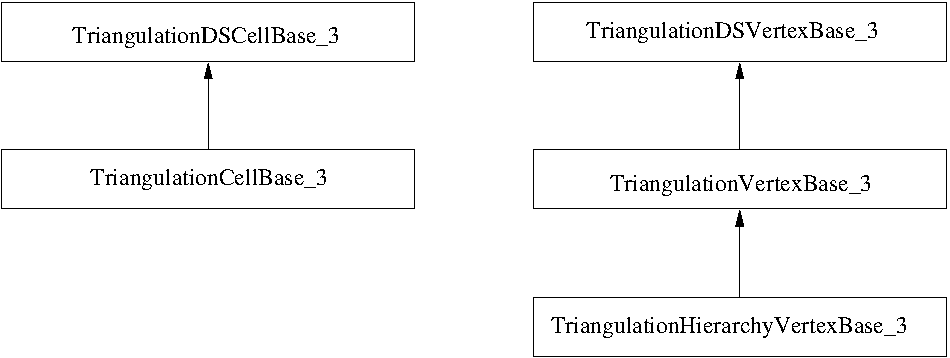
\includegraphics[width=13cm]{Triangulation_3/concept_hierarchy}
\end{center}
\end{ccTexOnly}
\begin{ccHtmlOnly}
<CENTER>
<img border=0 src="./concept_hierarchy.gif" align=middle
alt="Concepts refinement hierarchy for the vertex and cell base classes parameters">
</CENTER>
\end{ccHtmlOnly}
\caption{Concepts refinement hierarchy for the vertex and cell base classes
parameters.
\label{T3-concept-hierarchy}}
\end{figure}

A default value for the triangulation data structure parameter is provided in
all the triangulation classes, so it need not be specified by the user unless
he wants to use a different triangulation data structure or a different vertex
or cell base class.

\subsection{The Location Policy Parameter\label{Triangulation3-sec-locpol}}

The Delaunay triangulation class supports an optional feature which maintains
an additional data structure for fast point location queries.  
The fast location policy should be used when the user inserts points in a random
order or needs to do many unrelated queries.
If the user is able to give a good hint to help the point  location of
 its queries (and its newly inserted points), then it should prefer the default
 policy. In such a case where good hints are provided,
the default policy save some memory (few percents), and is faster.
Notice that if points are not inserted one by one, but as a  range, then a good hint is 
automatically computed using spatial sort.

Reading Section~\ref{Triangulation3-sec-complexity} on complexity and
performance can help making an informed choice for this parameter.

The point location strategy can be selected with the third template argument of
\ccc{Delaunay_triangulation_3}, \ccc{LocationPolicy}, which enables a fast
point location data structure when set to \ccc{Fast_location}.  By default, it
uses \ccc{Compact_location}.

Note that you can specify the \ccc{LocationPolicy} parameter without specifying
the triangulation data structure, in case you are fine with the default there.
In this case, the \ccc{LocationPolicy} appears as a second parameter after the
geometric traits.\footnote{The mechanism used behind the scenes to allow this
syntactical convenience is called \textit{deduced parameters}.} 

The \ccc{Fast_location} policy is implemented using a hierarchy of
triangulations; it changes the behavior of functions \ccc{locate},
\ccc{insert}, \ccc{move}, and \ccc{remove}.
As proved in~\cite{cgal:d-dh-02}, this structure has an
optimal behavior when it is built for Delaunay triangulations.

In this setting, if you build a triangulation by iteratively inserting points,
you should try to shuffle the points beforehand, as the time complexity is
guaranteed only for a randomized order.  For example, inserting points in
lexicographic order is typically much slower.  Note that this shuffling is
performed internally by the constructor taking a range of points.

Prior to \cgal\ 3.6, this functionality was available through the
\ccc{Triangulation_hierarchy_3} class, which is now deprecated.

\subsection{Flexibility of the Design}

In order to satisfy as many uses as possible, a design has been selected that
allows to exchange different parts to meet the users' needs, while still
re-using a maximum of the provided functionalities.  We have already seen that
the main triangulation classes are parameterized by a geometric traits class
and a triangulation data structure (TDS), so that each of them can be
interchanged with alternate implementations.

The most useful flexibility is the ability given to the user to add his own
data in the vertices and cells by providing his own vertex and cell base
classes to \ccc{Triangulation_data_structure_3}.  The
Figure~\ref{T3-fig-layers} shows in more detail the flexibility that is
provided, and the place where the user can insert his own vertex and/or cell
base classes.

\begin{figure}[htbp]
\begin{ccTexOnly}
\begin{center}
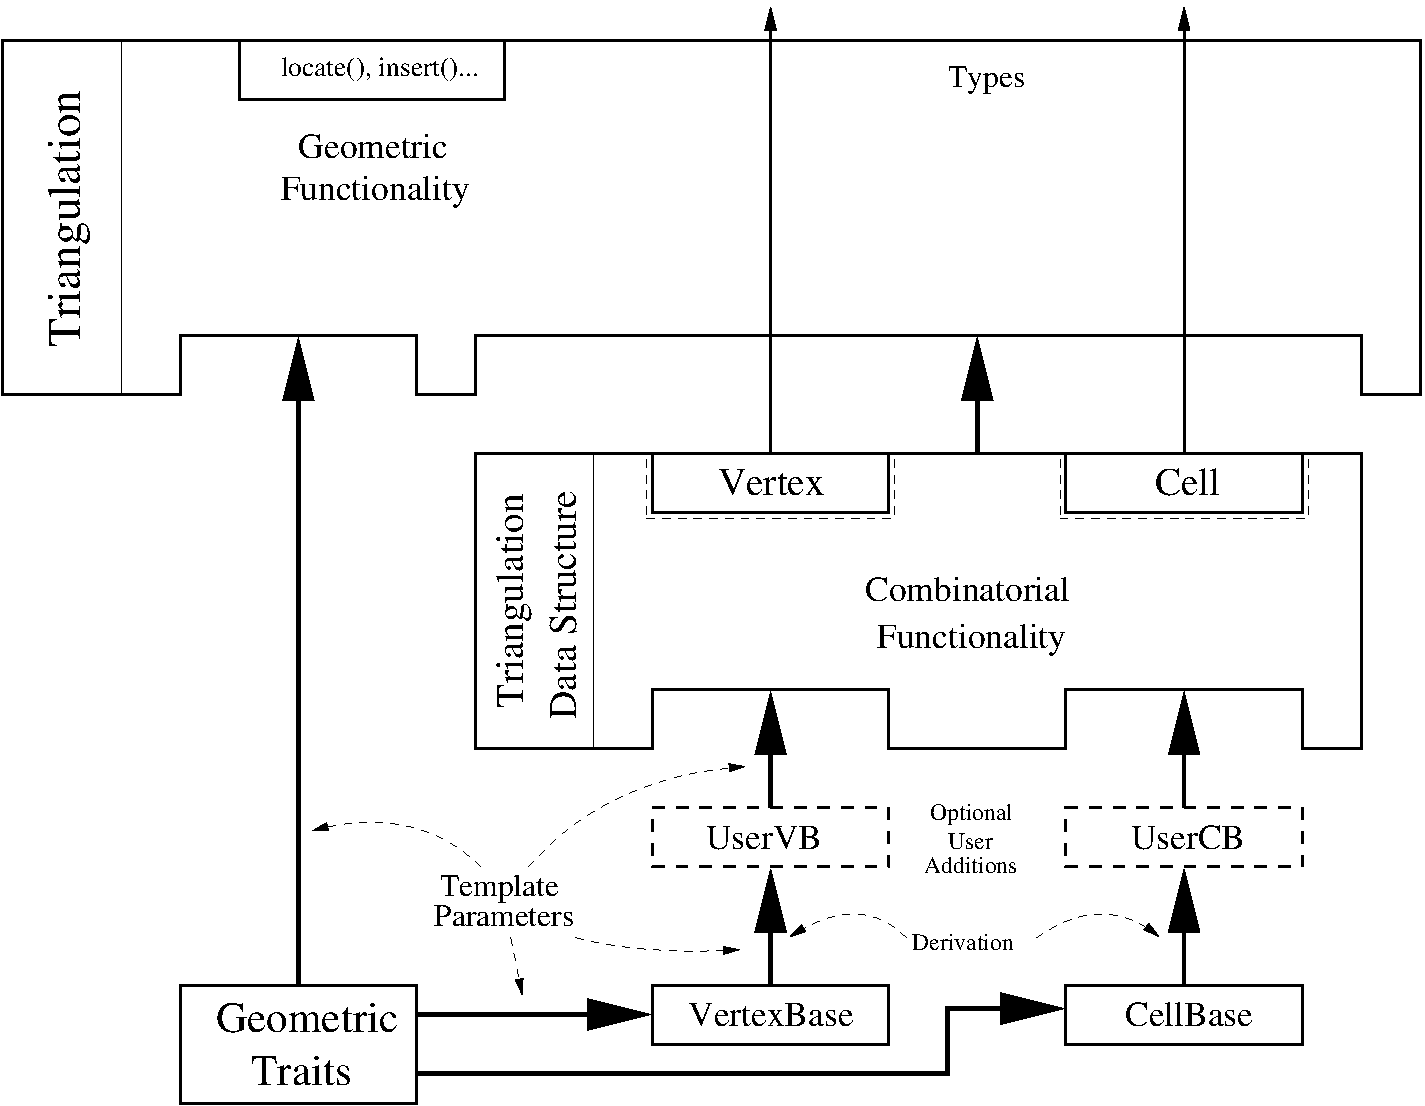
\includegraphics[width=13cm]{Triangulation_3/design}
\end{center}
\end{ccTexOnly}
\begin{ccHtmlOnly}
<CENTER>
<img border=0 src="./design.gif" align=middle alt="Triangulation software design">
</CENTER>
\end{ccHtmlOnly}
\caption{Triangulation software design.
\label{T3-fig-layers}}
\end{figure}


The design of the triangulation data structure gives the possibility to store
any kind of data, including handles (an entity akin to pointers) directly in
the vertex and cell base classes.

To do so, there are three possibilities.  The simplest one is to use the
class \ccc{Triangulation_vertex_base_with_info_3}, and this approach is
illustrated in a following subsection~\ref{Triangulation3-sec-examples-color}.
The most complicated one, and probably useless for almost all cases, is to
write a vertex base class from scratch, following the documented requirements.
This is mostly useless because most of the time it is enough to derive from
the models that \cgal\ provides, and add the desired features.
In this case, when the user needs to access some type that depends on the
triangulation data structure (typically handles), then he should write
something like:
\begin{ccExampleCode}
...
template < class GT, class Vb = Triangulation_vertex_base<GT> >
class My_vertex
  : public Vb
{
public:
  typedef typename Vb::Point           Point;
  typedef typename Vb::Cell_handle     Cell_handle;

  template < class TDS2 >
  struct Rebind_TDS {
    typedef typename Vb::template Rebind_TDS<TDS2>::Other  Vb2;
    typedef My_vertex<GT, Vb2>                             Other;
  };

  My_vertex() {}
  My_vertex(const Point&p)                : Vb(p) {}
  My_vertex(const Point&p, Cell_handle c) : Vb(p, c) {}
...
};
... // The rest has not changed
\end{ccExampleCode}

The situation is exactly similar for cell base classes.
Section~\ref{TDS3-sec-design} provides more detailed information.


\section{Examples\label{Triangulation3-sec-examples}}
\subsection{Basic Example}
This example shows the incremental construction of a 3D triangulation, the
location of a point and how to perform elementary operations on indices in a
cell. It uses the default parameter of the \ccc{Triangulation_3} class.

\ccIncludeExampleCode{Triangulation_3/simple_triangulation_3.cpp}

\subsection{Changing the Vertex Base}
The following two examples show how the user can plug his own vertex base in a
triangulation.  Changing the cell base is similar.

\subsubsection{Adding a Color\label{Triangulation3-sec-examples-color}}
When the user doesn't need to add a type in a vertex which depends on the
\ccc{TriangulationDataStructure_3} (e.g. a \ccc{Vertex_handle} or
\ccc{Cell_handle}), then he can use the
\ccc{Triangulation_vertex_base_with_info_3} class to add his own information
easily in the vertices.  The example below shows how to add a \ccc{CGAL::Color}
this way.

\ccIncludeExampleCode{Triangulation_3/color.cpp}

\subsubsection{Adding Handles}
When the user needs to add a type in a vertex which depends on the
\ccc{TriangulationDataStructure_3} (e.g. a \ccc{Vertex_handle} or
\ccc{Cell_handle}), then he has to derive his own vertex base class,
as the following example shows.

\ccIncludeExampleCode{Triangulation_3/adding_handles_3.cpp}

\subsection{Setting Information While Inserting a Range of Points}
The most efficient method to insert (weighted) points in a
Delaunay (or regular) triangulation is to provide an iterator
range over (weighted) points to the insert function. However, an iterator range of
(weighted) points does not allow to set different information to each vertex.
To solve this problem, in the case the vertex type  of the triangulation 
is a model of the concept \ccc{TriangulationVertexBaseWithInfo_3}
(such as \ccc{Triangulation_vertex_base_with_info_3}), we provide three examples 
doing the same operation: set an unsigned integer as the information 
of each vertex. The value of this unsigned integer is the initial order
of the corresponding point given in the range.

\subsubsection{Using an Iterator Over Pairs}
Each point and its information are gathered into a pair. We provide
the constructor of the triangulation (which is calling the \ccc{insert} function)
with a range of such pairs.
\ccIncludeExampleCode{Triangulation_3/info_insert_with_pair_iterator.cpp}


\subsubsection{Using the Boost Zip Iterator}

Information and points are in separate containers. We use
\ccAnchor{http://www.boost.org/libs/iterator/doc/index.html#specialized-adaptors}
{\ccc{boost::zip_iterator}} to provide an iterator gathering them.

\ccIncludeExampleCode{Triangulation_3/info_insert_with_zip_iterator.cpp}

\subsubsection{Using the Boost Transform Iterator}

We define a functor \ccc{Auto_count} used together with
 \ccAnchor{http://www.boost.org/libs/iterator/doc/index.html#specialized-adaptors}
{\ccc{boost::transform_iterator}} to set the order of each point
in the range. Note that this is correct because the iterator
is dereferenced only once per point during the insertion.
\ccIncludeExampleCode{Triangulation_3/info_insert_with_transform_iterator.cpp}


\subsection{The Simplex Class\label{Triangulation3-sec-simplex}}
The triangulation defines a \ccc{Simplex} class that represents a
simplex (vertex, edge, facet or cell). This example demonstrates how
simplices can be stored in a set.

\ccIncludeExampleCode{Triangulation_3/simplex.cpp}


\subsection{Fast Point Location for Delaunay Triangulations\label{Triangulation3-ex-fast-location}}

\ccIncludeExampleCode{Triangulation_3/fast_location_3.cpp}

\subsection{Finding the Cells in Conflict with a Point in a Delaunay
Triangulation}

\ccIncludeExampleCode{Triangulation_3/find_conflicts_3.cpp}

\subsection{Regular Triangulation}
This example shows the building of a regular triangulation.  In this
triangulation, points have an associated weight, and some points can
be hidden and do not result in vertices in the triangulation.
Another difference is that a specific traits class has to be used
(at least at the moment).

\ccIncludeExampleCode{Triangulation_3/regular_3.cpp}

\section{Complexity and Performance\label{Triangulation3-sec-complexity}}

In 3D, the worst case complexity of a triangulation is quadratic in the number
of points.  For Delaunay triangulations, this bound is reached in cases such as
points equally distributed on two non-coplanar lines.  However, the good news
is that, in many cases, the complexity of a Delaunay triangulation is linear or
close to linear in the number of points.  Several
articles~\cite{d-hdvdl-89,e-dpssdt-02,geometrica-5986i,prisme-4453a,prisme-abl-03}
have proved such good complexity bounds for specific point distributions, such
as points distributed on surfaces under some conditions.

\subsection{Running Time}

There are several algorithms provided in this package.  We will focus here on
the following ones and give practical numbers on their efficiency~:
\begin{itemize}
\item construction of a triangulation from a range of points, 
\item location of a point (using the \ccc{locate} function),
\item removal of a vertex (using the \ccc{remove} function).
\end{itemize}

We will use the following types of triangulations, using
\ccc{Exact_predicates_inexact_constructions_kernel} as geometric traits
(combined with \ccc{Regular_triangulation_euclidean_traits_3} in the weighted
case)~:
\begin{itemize}
\item \textbf{Delaunay} : \ccc{Delaunay_triangulation_3}
\item \textbf{Delaunay - Fast location} : \ccc{Delaunay_triangulation_3} with \ccc{Fast_location}
\item \textbf{Regular} : \ccc{Regular_triangulation_3} (default setting : memorize hidden points)
\item \textbf{Regular - No hidden points} : \ccc{Regular_triangulation_3} with hidden points discarded (using
      \ccc{Triangulation_cell_base_3} instead of \ccc{Regular_triangulation_cell_base_3}).
\end{itemize}

Figure~\ref{Triangulation3-fig-benchmarks} shows, for all these types of
triangulations, the times in seconds taken to build a triangulation from a
given number of points, then the average time to perform one point location in
triangulations of various sizes, and the average time to perform one vertex
removal (which is largely independent on the size of the triangulation).

The data sets used here are points randomly distributed in the unit cube (the
coordinates are generated using the \texttt{drand48} C function).  In the
weighted case, the weights are all zero, which means that there are actually no
hidden points during execution.

The measurements have been performed using \cgal\ 3.6, using the \gnu\ \CC\ compiler
version 4.3.2, under Linux (Fedora 10 distribution), with the compilation options
\texttt{-O3 -DCGAL\_NDEBUG}.  The computer used was equipped with a 64bit Intel
Xeon 3GHz processor and 32GB of RAM (a recent desktop machine as of 2009).
% Note : it's "tigre" that I used.

\begin{figure}[htbp]
\begin{center}
\begin{tabular}{|l||r|r|r|r|}
\hline
& \textbf{Delaunay} & \textbf{Delaunay}      & \textbf{Regular} & \textbf{Regular} \\
&                   & \textbf{Fast location} &                  & \textbf{No hidden points} \\
\hline\hline
Construction from $10^2$ points & 0.00054 & 0.000576 & 0.000948 & 0.000955 \\
Construction from $10^3$ points & 0.00724 & 0.00748  & 0.0114   & 0.0111\\
Construction from $10^4$ points & 0.0785  & 0.0838   & 0.122    & 0.117 \\
Construction from $10^5$ points & 0.827   & 0.878    & 1.25     & 1.19 \\
Construction from $10^6$ points & 8.5     & 9.07     & 12.6     & 12.2 \\
Construction from $10^7$ points & 87.4    & 92.5     & 129      & 125 \\
\hline
Point location in $10^2$ points & 9.93e-07 & 1.06e-06 & 7.19e-06 & 6.99e-06 \\
Point location in $10^3$ points & 2.25e-06 & 1.93e-06 & 1.73e-05 & 1.76e-05 \\
Point location in $10^4$ points & 4.79e-06 & 3.09e-06 & 3.96e-05 & 3.76e-05 \\
Point location in $10^5$ points & 2.98e-05 & 6.12e-06 & 1.06e-04 & 1.06e-04 \\
Point location in $10^6$ points & 1e-04    & 9.65e-06 & 2.7e-04  & 2.67e-04 \\
Point location in $10^7$ points & 2.59e-04 & 1.33e-05 & 6.25e-04 & 6.25e-04 \\
\hline
Vertex removal                  & 1e-04    & 1.03e-04 & 1.42e-04 & 1.38e-04 \\
\hline
\end{tabular}
\end{center}
\caption{Running times in seconds for algorithms on 3D triangulations.
\label{Triangulation3-fig-benchmarks}}
\end{figure}

More benchmarks comparing \cgal\ to other software can be found
in~\cite{msri52:liu-snoeyink-05}.


\subsection{Memory Usage}

We give here some indication about the memory usage of the triangulations.
Those structures being intensively based on pointers, the size almost doubles
on 64bit platforms compared to 32bit.

The size also depends on the size of the point type which is copied in the
vertices (hence on the kernel).  Obviously, any user data added to vertices
and cells also affect the memory used.

More specifically, the memory space used to store a triangulation is first
a function of the size of its \ccc{Vertex} and \ccc{Cell} types times their
numbers (and for volumic distribution, one sees about 6.7 times more cells than
vertices).  However, these are stored in memory using \ccc{Compact_container},
which allocates them in lists of blocks of growing size, and this requires some
additional overhead for bookkeeping.  Moreover, memory is only released to the
system when clearing or destroying the triangulation.  This can be important
for algorithms like simplifications of data sets which will produce fragmented
memory usage (doing fresh copies of the data structures are one way out in such
cases).  The asymptotic memory overhead of \ccc{Compact_container} for its
internal bookkeeping is otherwise on the order of $O(\sqrt{n})$.

Figure~\ref{Triangulation3-fig-memory} shows the number of bytes used per
points, as measured empirically using \ccc{Memory_sizer} for large triangulations
($10^6$ random points).

\begin{figure}[htbp]
\begin{center}
\begin{tabular}{|l||r|r|r|r|}
\hline
& \textbf{Delaunay} & \textbf{Delaunay}      & \textbf{Regular} & \textbf{Regular} \\
&                   & \textbf{Fast location} &                  & \textbf{No hidden points} \\
\hline\hline
32bit & 274 & 291 & 336 & 282 \\
\hline
64bit & 519 & 553 & 635 & 527 \\
\hline
\end{tabular}
\end{center}
\caption{Memory usage in bytes per point for large data sets.
\label{Triangulation3-fig-memory}}
\end{figure}


\subsection{Variability Depending on the Data Sets and the Kernel}

Besides the complexity of the Delaunay triangulation that varies with the
distribution of the points, another critical aspect affects the efficiency~:
the degeneracy of the data sets.  These algorithms are quite sensitive to
numerical accuracy and it is important to run them using exact predicates.

Using a kernel with no exact predicates will quickly lead to crashes or
infinite loops once they are executed on non-random data sets.  More precisely,
problems appear with data sets which contain (nearly) degenerate cases for the
\ccc{orientation} and \ccc{side_of_oriented_sphere} predicates, namely when
there are (nearly) coplanar or (nearly) cospherical points.  This unfortunately
happens often in practice with data coming from various kinds of scanners or
other automatic acquisition devices.

Using an inexact kernel such as \ccc{Simple_cartesian<double>} would lead
to optimal performance, which is only about 30\% better than
\ccc{Exact_predicates_inexact_constructions_kernel}.  The latter is strongly
recommended since it takes care about potential robustness issues.  The former
can be used for benchmarking purposes mostly, or when you really know that your
data sets won't exhibit any robustness issue.

Exact predicates take more time to compute when they hit (nearly) degenerate
cases.  Depending on the data set, this can have a visible impact on the
overall performance of the algorithm or not.

Sometimes you need exact constructions as well, so
\ccc{Exact_predicates_exact_constructions_kernel} is a must.  This is the case
for example when you need the \ccc{dual} functions to be exact, or when your
input is stored in points of such a kernel for other reasons (because it is the
output of another algorithm which has this requirement, for example).  This
will slow down the computations by a factor of 4 to 5 at least, and it can be
much more.

Figure~\ref{Triangulation3-fig-kernels-and-data-sets} gives more detailed
timings about various kernels one the following data sets~: random points in a
cube, random points on the surface of an ellipsoid, points scanned on the
surface of a Buddha statue, points on a molecular surface, and points scanned
on a dryer handle.  See Figure~\ref{Triangulation3-fig-data-sets} for pictures of
the last 3 objects, which respectively illustrate volumic data, surfacic data,
and data with many degenerate cases.  This last data set exhibits an infinite
loop with an inexact kernel, and of course we are not sure whether what is
computed for the other data sets with this inexact kernel is a Delaunay
triangulation.  General introductory information about these robustness issues
can be found in~\cite{cgta-kmpsy-08}.  More benchmarks around this issue can
also be found in~\cite{cgal:dp-eegpd-03}.

\begin{figure}[htbp]
\begin{center}
\begin{tabular}{|l||r|r|r|r|r|}
\hline
         & \textbf{Random} & \textbf{Ellipsoid} & \textbf{Buddha} & \textbf{Molecule} & \textbf{Dryer} \\
         &                 &                    &                 &                   & \textbf{Handle} \\
\#points & \textbf{100000} & \textbf{100000}    & \textbf{542548} & \textbf{525296}   & \textbf{49787} \\
\hline\hline
\ccc{Simple_cartesian<double>} & 0.69 & 0.627 & 4.21 & 3.8 & $\infty$-loop \\
\hline
\ccc{Exact_predicates_inexact_constructions_kernel} & 0.824 & 0.749 & 4.99 & 4.64 & 1.68 \\
\hline
\ccc{Exact_predicates_exact_constructions_kernel} & 4.59 & 3.85 & 30.1 & 26.4 & 4.57 \\
\hline
\ccc{Simple_cartesian<Gmpq>}   & 492 & 534 & 1120 & 1030 & 75.2 \\
\hline
\end{tabular}
\end{center}
\caption{Running times (seconds) for various kernels and data sets.
\label{Triangulation3-fig-kernels-and-data-sets}}
\end{figure}


\begin{figure}[htbp]
\begin{center} 
\begin{ccTexOnly}
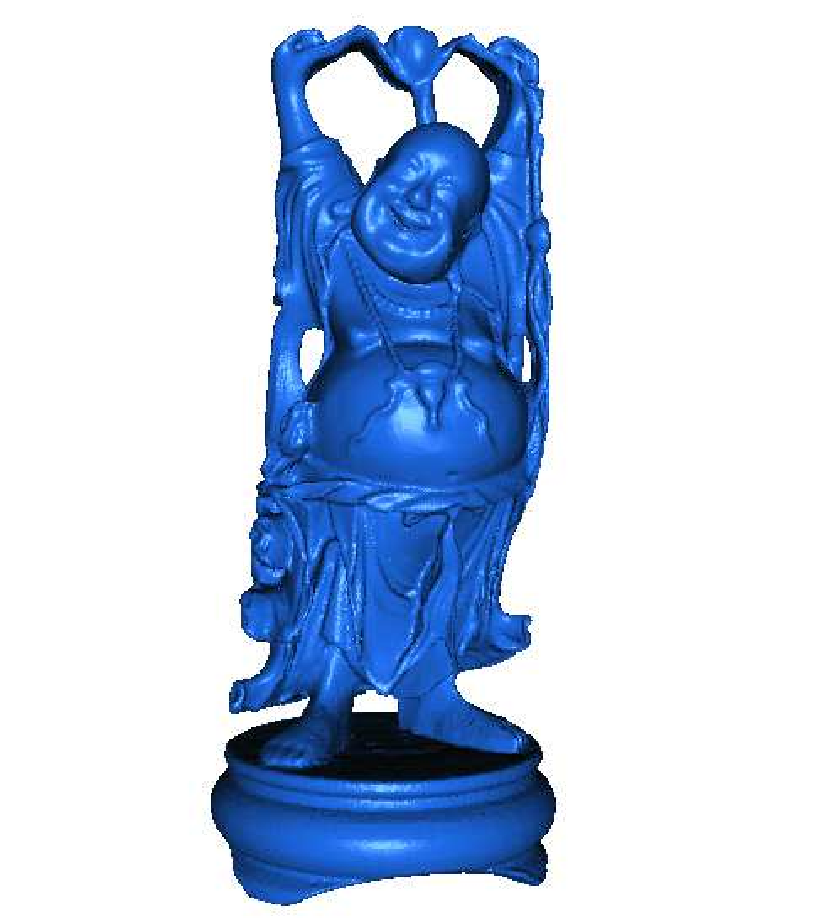
\includegraphics[width=5cm]{Triangulation_3/fig/api1_01} 
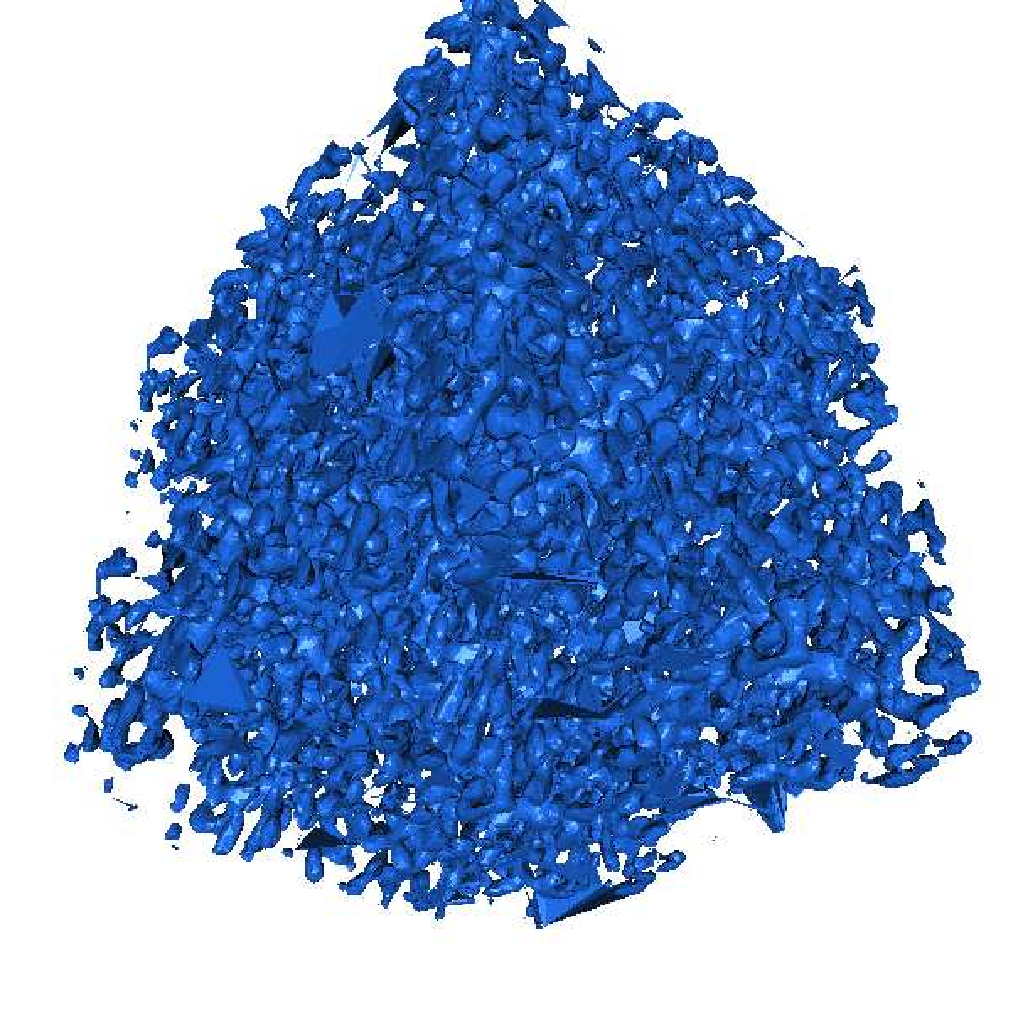
\includegraphics[width=5cm]{Triangulation_3/fig/b35-1} 
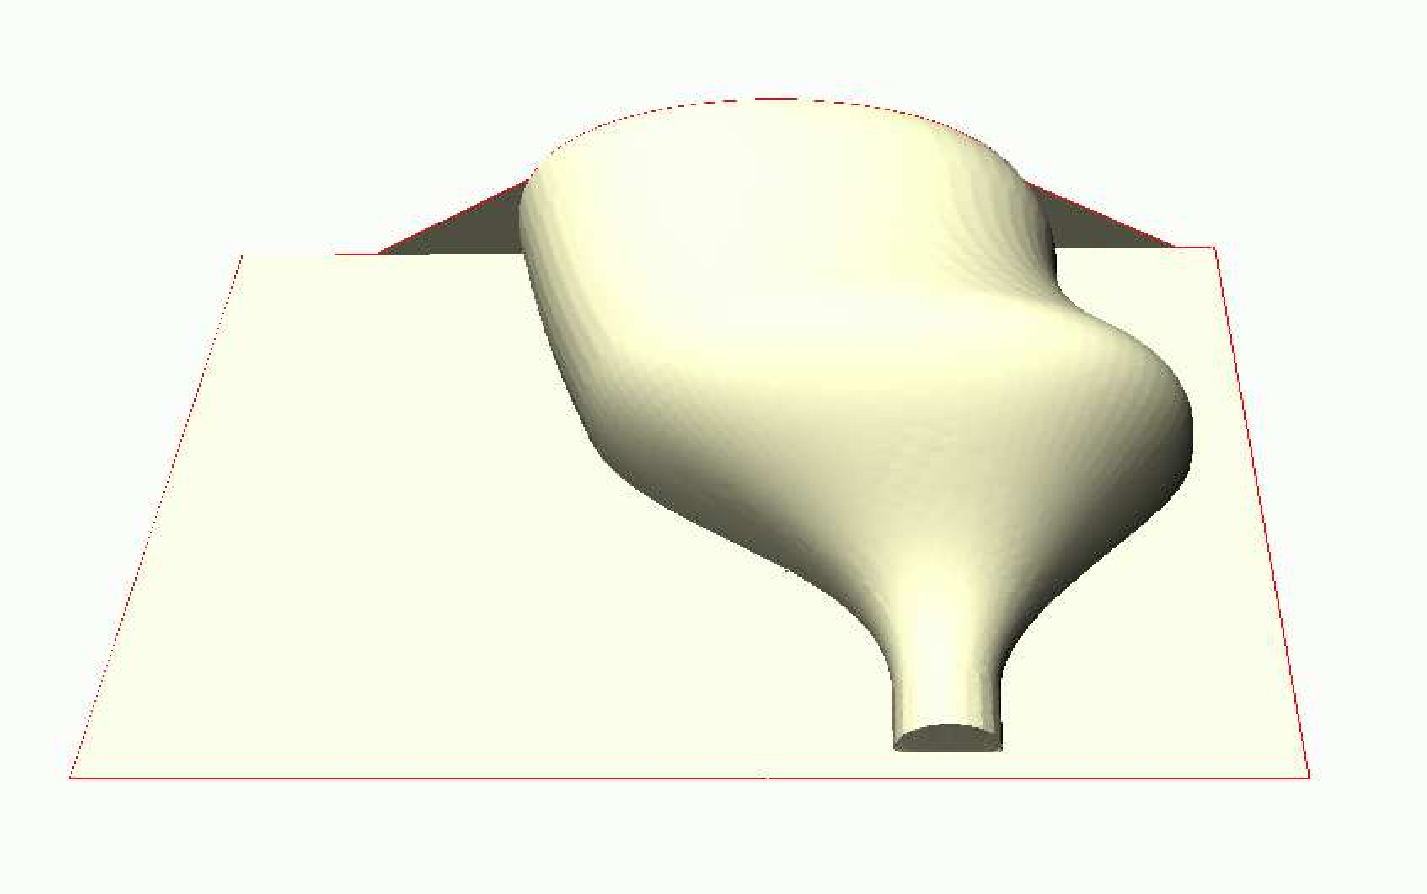
\includegraphics[width=5cm]{Triangulation_3/fig/HD} 
\end{ccTexOnly}
\begin{ccHtmlOnly}
<table>
<tr>
<td width="30%"><img border=0 width="100%" src="./fig/api1_01.gif" alt="Buddha statue">
<td width="30%"><img border=0 width="100%" src="./fig/b35-1.gif" alt="Molecule">
<td width="30%"><img border=0 width="100%" src="./fig/HD.gif" alt="Dryer Handle">
</table>
\end{ccHtmlOnly}
\end{center}
\caption{Data sets used in the benchmark of Figure~\ref{Triangulation3-fig-kernels-and-data-sets}.
\label{Triangulation3-fig-data-sets}}
\end{figure} 



%%%%%%%%%%%%%%%%%%%%%%%%%%%%%%%%
\section{Design and Implementation History}

Monique Teillaud started to work on the 3D triangulation packages in
1997, following the design of the 2D triangulation packages. The
notions of degenerate dimensions and infinite vertex were formalized
\cite{t-tdtc-99} and induced changes in the 2D triangulation
packages. The packages were first released in \cgal\ 2.1. They contained
basic functionalities on triangulations, Delaunay triangulations,
regular triangulations.

A first version of removal of a vertex from a Delaunay triangulation
was released in \cgal\ 2.2. However, this removal became really robust
only in \cgal\ 2.3, after some research that allowed to deal with
degenerate cases quite easily \cite{cgal:dt-pvr3d-03}. Andreas Fabri
implemented this revised version of the removal, and a faster removal
algorithm for \cgal\ 3.0. 

The latter algorithm was proposed by Mariette Yvinec, who contributed
in several ways to the package, first since she was maintaining the
close 2D triangulation package and participated in many discussions,
she also wrote the traits classes for regular triangulations.

In 2000, Sylvain Pion started working on these packages.  He improved
the efficiency of triangulations in \cgal\ 2.3 and 2.4 in several ways
\cite{cgal:bdpty-tc-02}: he implemented the Delaunay hierarchy
\cite{cgal:d-dh-02} in 2.3, he improved the memory footprint in 2.4
and 3.0, he also performed work on arithmetic filters
\cite{cgal:dp-eegpd-03} (see \ccc{Filtered_kernel}) to improve
the speed of triangulations.  He changed the design in \cgal\ 3.0,
allowing users to add handles in their own vertices and cells.

Olivier Devillers, co-author of preliminary versions of the \cgal\ 2d
triangulations, participated in many discussions, in particular about
the perturbations, and more concretely in the implementation of the
Delaunay hierarchy. 

In 2005, Christophe Delage implemented the vertex removal function for
regular triangulations, using the symbolic perturbation proposed
in~\cite{cgal:dt-pvrdr-06}, which allowed to release this
functionality in \cgal\ 3.2.

In 2006, Nico Kruithof wrote the \ccc{Triangulation_simplex_3} class
that can store simplices of any dimension and improved the internal 
organization of the code.

As of March 2007, Christophe Delage made the iterator range insert methods and
constructors use \ccc{spatial_sort} to improve efficiency.

In 2008, Camille Wormser added a few more iterators in
the package that were integrated in release~3.4.

In 2009, Sylvain Pion simplified the design of the Delaunay hierarchy
so that it became the simple \ccc{Fast_location} policy in release~3.6.

In 2010, Pedro de Castro and Olivier Devillers added the point
displacement in release 3.7.

In 2011,  Pedro de Castro and Olivier Devillers implemented in release
3.8 the
structural filtering method, improving the efficiency of point location.

A new demo of this package was introduced in CGAL 3.8, coded by Fei
(Sophie) Che, who was co-mentored by Manuel Caroli and Monique
Teillaud in the framework of the Google Summer of Code, 2010.

The authors wish to thank Lutz Kettner for inspiring discussions about
the design of CGAL. Jean-Daniel Boissonnat is also acknowledged
\cite{bdty-tcgal-00}.
